\documentclass[lang=cn,10pt,chinesefont=founder,toc=twocol]{elegantbook}

\title{概率论笔记}
%\subtitle{}

\author{肖程哲}
%\institute{}
\date{\today}
%\version{}
%\bioinfo{自定义}{信息}

\extrainfo{苟日新,日日新,又日新}

\setcounter{tocdepth}{3}

\logo{logo.png}
\cover{cover.jpg}

% 本文档命令
\usepackage{array, fdsymbol, float, bbm,tabularx,booktabs,multirow,bm,subcaption}
\usetikzlibrary{decorations.pathreplacing,decorations.pathmorphing,arrows.meta,patterns}
\usepackage[below]{placeins}
\usepackage[free-standing-units]{siunitx}

\newcommand{\ucite}[1]{\textsuperscript{\cite{#1}}}
% 参考文献引用:上标用 \ucite{ }, 文中用 \cite{ }
\newcommand{\red}[1]{{\color{red}#1}}

\newcommand{\widesim}[2][1.5]{
	\mathrel{\overset{#2}{\scalebox{#1}[1]{$\sim$}}}
}
\newcommand{\iidsim}{\widesim[2.33]{\mathrm{i.i.d.}}}	% independent and identically distributed
\newcommand{\indep}{\Vbar}		% independent
\newcommand{\X}{\mathcal{X}}		% 
\newcommand{\1}{\mathbbm{1}}				% indicator
\renewcommand{\P}{\mathbb{P}}				% probability
\newcommand{\as}{\mathrm{a.s.}}				% almost surely
\newcommand{\E}{\mathbb{E}}					% expectation
\newcommand{\Var}{\operatorname{Var}}		% variance
\newcommand{\Cov}{\operatorname{Cov}}		% covariance
\newcommand{\Cor}{\operatorname{Cor}}		% covariance
\newcommand{\MSE}{\operatorname{MSE}}		% mean square error
\newcommand{\mean}[1]{\overline{#1}}
\newcommand{\abs}[1]{\left\lvert#1\right\rvert}		% absolute value
\newcommand{\norm}[1]{\left\lVert#1\right\rVert}
\newcommand{\rank}[1]{\operatorname{rank}\left(#1\right)}
\newcommand{\tr}[1]{\operatorname{tr}\left(#1\right)}		% trace
\newcommand{\diag}[1]{\operatorname{diag}\!\left(#1\right)}			% diagonal
\newcommand{\vspan}[1]{\operatorname{span}\left(#1\right)}	% vector span
\newcommand{\proj}[2]{\operatorname{proj}_{#2}#1}			% projection
\newcommand{\inprod}[2]{\left\langle #1, #2 \right\rangle}	% inner product
\newcommand{\R}{\mathbb{R}}					% real
\renewcommand{\Rn}{\mathbb{R}^n}				% real n dimensions
\renewcommand{\d}{\mathrm{d}}				% differential
\newcommand{\pd}{\partial}					% partial differential
\newcommand{\p}[3][]{\frac{\pd^{#1}#2}{\pd{#3}^{#1}}}	% partial derivative
\newcommand{\e}{\varepsilon}
\newcommand{\st}{\mathrm{s.t.}\ }			% subject to, so that
\newcommand{\argmin}{\operatornamewithlimits{arg\,min}}
\newcommand{\argmax}{\operatornamewithlimits{arg\,max}}
\newcommand{\N}{\mathcal{N}}				% normal, not natural numbers XD
\newcommand{\ee}{\mathrm e}
\newcommand{\dd}{\mathop{}\!\mathrm d}
\newcommand{\textop}[1]{\relax\ifmmode\mathop{\text{#1}}\else\text{#1}\fi}
\newcommand{\TT}{^{\mathrm T}}

\renewcommand\arraystretch{2}

\setlist[description]{
	labelindent = 3em,
	labelwidth = 7em,
	leftmargin = 10em,
	labelsep = 0em,
	parsep = 0.75em,
	topsep = 0.75em,
}

\includeonly{appendix/Appendix}
\begin{document}

\maketitle
\frontmatter
\tableofcontents

\mainmatter
\chapter{概率基础}

\begin{introduction}
    \item 事件
    \item 古典概型与几何概率
    \item 条件概率与独立
    \item 乘法法则
    \item 全概率公式
    \item Bayes法则
\end{introduction}

\section{概率空间}

\begin{definition}[样本空间]
    随机试验可能出现的结果称为\textbf{样本点}(sample point),用$\omega$表示。样本的全体构成\textbf{样本空间}(sample space),用$\Omega$表示。
\end{definition}

\begin{definition}[事件的古典定义]
    样本点$\omega$的集合称为\textbf{事件}(event)。
\end{definition}

我们关心的随机现象被抽象为集合, 逻辑运算(且, 或, 非, etc.)对应成集合论运算(交, 并, 补, etc.)。

\begin{property}
    集合的运算性质:
    \begin{description}
        \item [交换律] $A \cup B = B \cup A, \quad AB = BA$
        \item [结合律] $(A \cup B) \cup C = A \cup (B \cup C), (AB)C = A(BC)$
        \item [分配律]
              \begin{gather}
                  (A \cup B) \cup C = A \cup (B \cup C),\\
                  (A \cap B) \cup C = (A \cup C) \cap (B \cup C).
              \end{gather}
        \item [对偶律(De Morgan's laws)]
              \begin{gather}
                  \text{事件并的对立等于对立的交:} \quad \overline{A \cup B} = \overline{A} \cap \overline{B},\\
                  \text{事件交的对立等于对立的并:} \quad \overline{A \cap B} = \overline{A} \cup \overline{B}.
              \end{gather}
    \end{description}
\end{property}

为方便概率的定义,并不把$\Omega$的一切子集作为事件,应避免不可测集的出现。

\begin{definition}[事件域]
    事件构成的全体称为\textbf{事件域}$\mathscr{F}$,是$\Omega$的子集族(collection of subsets),应满足\underline{\,$\sigma$代数}的要求:
    \begin{itemize}
        \item $\emptyset \in \mathscr{F}$, 无事发生;
        \item $A\in\mathscr{F} \implies A^{\complement}\in\mathscr{F}$, 即$\mathscr{F}$对补集运算(逻辑上的非)封闭;
        \item $A_{1},\dots,A_{n},\ldots \in \mathscr{F} \implies \bigcap_{n=1}^{\infty}A_{n} \in \mathscr{F}$, 即$\mathscr{F}$对可数交运算(逻辑上的可数多个且)封闭.
    \end{itemize}
\end{definition}

\begin{note}
    可数性是为了在数学上能够恰当地处理\underline{无穷}的概念, 术语中的$\sigma$指的就是\underline{可数并}。由对偶原理可得$\sigma$域同时对可数并运算封闭. 即$\sigma$域对逆, 并, 交, 差的可数次运算封闭.
\end{note}

事件域根据问题的不同要求适当选取, 在概率定义没有困难时, 应尽量选大, 通常以$\Omega$的一切子集作为事件域. 当$\Omega$给定后,若某些子集必须作为事件处理, 能否找到包含他们的$\sigma$域?

\begin{proposition}
    若给定$\Omega$的一个非空集族$\mathscr{G}$, 必存在$\Omega$上唯一的$\sigma$域$\mathfrak{m}(\mathscr{G})$, 满足下列性质:
    \begin{itemize}
        \item 包含$\mathscr{G}$
        \item 若其他$\sigma$域包含$\mathscr{G}$, 则必包含$\mathfrak{m}(\mathscr{G})$
    \end{itemize}
    这个$\mathfrak{m}(\mathscr{G})$称为包含$\mathscr{G}$的最小$\sigma$域, 或由$\mathscr{G}$扩张而成的$\sigma$域.
\end{proposition}

\emph{扩张}, 或者称为\emph{延拓}, 是数学中很重要的一个概念, 大抵是将某映射的定义域适当扩大, 不改变在初始定义域上的映射取值(注意值域可能是比较抽象的集合, 配备了某些操作之后被称为空间), 同时在扩大后的定义域上仍然保持某些优良的性质. 与此相对的概念是\emph{限制}, 即关心局部上可能更加漂亮的性质, 把初始的定义域适当缩小.

\begin{proof}
    由于$\Sigma$的一切子集构成的集类包含$\mathscr{G}$, 所以$\mathfrak{m}$存在. 再取$\Sigma$上满足此条件的$\sigma$域之交作为$\mathfrak{m}(\mathscr{G})$即可.
\end{proof}

特别地, 实数集$\R$的子集族$\{(-\infty,x] : x\in\R\}$生成的$\sigma$代数$\mathscr{B}_{\R}$称为$\R$上的\emph{Borel代数}.

\begin{definition}[Borel集]
    设$\mathbb{R}^1$为全集, 形为$[a,b)$构成的集类产生的$\sigma$域称为\textbf{一维Borel$\sigma$域}, 记为$\mathscr{B}_1$, 其中的元素称为\textbf{一维Borel集}
\end{definition}

若$x,y$为任意实数,由于:
\begin{align*}
    \{x\}  & =  \bigcap_{n=1}^{\infty}\left[x, x+\frac{1}{n}\right) \\
    (x, y) & =  [x, y)-\{x\}                                        \\
    [x, y] & =  [x, y)+\{y\}                                        \\
    (x, y] & =  [x, y)+\{y\}-\{x\}
\end{align*}
因此$\mathscr{B}_1$包含一切开区间, 闭区间, 单个实数, 可列个实数, 以及他们经可列次逆, 并, 交, 差运算的集合.

\begin{definition}[概率空间]
    定义在\underline{事件域}(非样本空间)上的集合函数$P : \mathscr{F} \to \mathbb{R}$称为\textbf{概率}的条件是:
    \begin{description}
        \item[非负性] $P(A)\ge 0 , \forall A \in \mathscr{F}$
        \item[规范性] $P(\Omega) = 1$; (如果没有这条就是一般的{\color{lightgray}有限}\emph{测度})
        \item[可列可加性] 若$A_{1},\dots,A_{n},\ldots \in \mathscr{F}$两两不交, 即$A_{i}\cap A_{j} = \emptyset, \ \forall i\neq j$, 则$P(\bigcup_{n=1}^{\infty}A_{n}) = \sum_{n=1}^{\infty}P(A_{n})$.
    \end{description}
    我们称$(\Omega,\mathscr{F},P)$为一个\textbf{概率空间}(probability space)
\end{definition}

\begin{property}
    概率的性质:
    \begin{itemize}
        \item $P(\Omega)=1$;
        \item $P(A^{\complement})=1-P(A)$;
        \item 若$A \subseteq B $ 则 $P(A)\le P(B)$;
    \end{itemize}
\end{property}

\begin{corollary}[加法公式]
    基础形式:
    \[ P(A \cup B) = P(A) + P(B) - P(AB) \]
    一般形式:
    \begin{align*}
         & P\left(A_{1} \cup A_{2} \cup \cdots \cup A_{n}\right) =  \sum_{i=1, \cdots, n} P\left(A_{i}\right)-\sum_{\substack{i<j \\
        i, j=1, \cdots, n}} P\left(A_{i} A_{j}\right)                                                                             \\
         & +\sum_{\substack{i<j<k                                                                                                 \\i, j, k=1, \cdots, n}} P\left(A_{i} A_{j} A_{k}\right)-\cdots+(-1)^{n-1} P\left(A_{1} A_{2} \cdots A_{n}\right)
    \end{align*}
    特别地, 若事件出现个数相同时概率相等,则可简化为:
    \[ P\left(A_{1} \cup A_{2} \cup \cdots \cup A_{n}\right)=n P_{1} - \binom{n}{2} P_{2} + \binom{n}{3} P_{3}- \cdots+(-1)^{n-1} P_{n} \]
\end{corollary}

显然,可列可加性可以推出有限可加性. 但是一般来讲,由有限可加性并不能推出可列可加性. 设$A_i \in \mathscr{F}, i=1,2,\cdots $且两两互不相容, 若希望由有限可加性推出可列可加性,则需要下式成立:
\[ \lim_{n \to \infty}P(\sum_{i=1}^n A_i) =P(\lim_{n \to \infty}\sum_{i=1}^{n} A_i) \]

\begin{definition}
    对于$\mathscr{F}$上的集合函数$P$,若它对$\mathscr{F}$中任何一个单调不减的集序列$\{ S_n \}$(即$ S_n \in \mathscr{F}, S_n \subseteq  S_{n+1} $)均满足:
    \[ \lim_{n \to \infty}P(S_n) =P(\lim_{n \to \infty} S_n) \]
    则称它是\textbf{下连续的}.
\end{definition}

故若令$S_n = \sum_{i=1}^n A_n$, 则可列可加性条件等价于有限可加性加下连续.

\section{古典概型与几何概型}

\subsection{古典概型}

\subsection{几何概型}

古典概型的基本思想:
\begin{description}
    \item[有限个样本点] 所涉及的随机现象只有有限个样本点, 譬如为 $n$ 个, 且这些事件是两两互不相容的;
    \item[等可能性] 每个样本点发生的可能性相等
\end{description}

\begin{definition}
    若事件 $A$ 含有 $k$ 个样本点, 则事件 $A$ 的概率为
    \[  P (A) = \frac{\text{事件 } A \text{ 所含样本点的个数}}{\Omega \text{ 中所有样本点的个数}} = \frac{k}{n} \]
\end{definition}

\begin{note}
    事实上,古典概型的大部分问题都能形象化地用摸球模型来描述以后我们经常研究摸球模型,意义即在于此.
\end{note}

\section{条件概率}

\begin{definition}[条件概率]
    令$A,B \in \mathscr{F}$, 且$P(B)>0$称
    \[ P(A|B) = \frac{P(A \cap B)}{P(B)}\]
    为\textbf{基于于$B$的条件概率}(probability conditional on $B$), 这仍然是一个概率测度.
\end{definition}

\begin{theorem}[乘法法则]
    令$A,B \in \mathscr{F}$, 且$P(B)>0$, 则
    \[ P(A \cap B) = P(A|B)P(B) \]
    泛化后有:
    \[ P(A_1 \cap A_2 \cap \cdots \cap A_n) = P(A_{1})P(A_2|A_1)P(A_3|A_1\cap A_2) \cdots  \]
\end{theorem}

\begin{theorem}[全概率公式]
    设 $B_1, B_2, \dotsc, B_n$ 为样本空间 $\Omega$ 的一个分割, 且互不相容, 即$\bigcup _{i=1} ^n B_i = \Omega, B_i B_j= \emptyset for i \neq j $
    如果 $P(B_i) > 0$, $i=1, 2, \dotsc, n$,
    则对任一事件 $A$ 有
    \begin{equation}
        P(A) = \sum_{i=1}^n P(B_i) P(A | B_i).
    \end{equation}
\end{theorem}

\begin{note}
    $P(A | B_i)$可视为事件$A$在$B_i$上的平均, $P(B_i)$则为其权重.
\end{note}

\begin{theorem}[Bayes定理]
    设 $B_1, B_2, \dotsc, B_n$ 为样本空间 $\Omega$ 的一个分割, 且互不相容, 即$\bigcup _{i=1} ^n B_i = \Omega, B_i B_j= \emptyset for i \neq j $
    如果 $P(A) > 0$, $P(B_i) > 0$, $i = 1,2, \dotsc, n$,
    则
    \begin{equation}
        P (B_i | A) = \frac{P(B_i) P(A|B_i)}{\sum_{j=1}^n P(B_j) P(A|B_j)}
    \end{equation}
\end{theorem}

\begin{definition}[事件的独立性]
    如果$A,B\in\mathscr{F}$满足
    \[ P(A\cap B) = P(A)P(B), \]
    则称$A$与$B$\textbf{独立}(independent), 记为$A \Vbar B$.

    对于事件集$A_1, A_2, \dotsc, A_n$, 若对于其中任意子集$A_{i_1}, A_{i_2}, \dotsc, A_{i_n}$有:
    \[ P(A_{i_1} \cap \cdots  \cap A_{i_n}) =P(A_{i_1})\cdots P(A_{i_n})  \]
    则称此事件集\textbf{相互独立}(mutually independent)
\end{definition}

\begin{note}
    当$P(A)>0$时, 我们有$ P(B|A) = P(B) \iff B \Vbar A$, 由此可得到\underline{$B$独立于$A$}的直观理解
\end{note}

\begin{property}
    独立性是对称的, 即$A \Vbar B \iff B \Vbar A$. 若两事件独立, 则其补集也独立.
    \begin{center}
        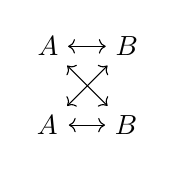
\begin{tikzpicture}
            \node[draw=none,fill=none] (1) at(0,0) {$A^{\complement}$};
            \node[draw=none,fill=none] (2) at(1,0) {$B^{\complement}$};
            \node[draw=none,fill=none] (3) at(0,1) {$A$};
            \node[draw=none,fill=none] (4) at(1,1) {$B$};
            \draw[<->] (1)--(2);
            \draw[<->] (1)--(4);
            \draw[<->] (3)--(2);
            \draw[<->] (3)--(4);
        \end{tikzpicture}
    \end{center}
\end{property}

\begin{definition}[事件域的独立性]
    若$\mathscr{G} \subset \mathscr{F}$与$\mathscr{H} \subset \mathscr{F}$满足
    \[ A \Vbar B, \quad \forall A\in\mathscr{G},\ B\in\mathscr{H}, \]
    则称$\mathscr{G}$与$\mathscr{H}$独立, 记为$\mathscr{G} \Vbar \mathscr{H}$
\end{definition}

测度论告诉我们一个重要结果: 如果$\mathscr{G}$对交集运算封闭, 那么成立$\mathscr{G}\Vbar\mathscr{H} \implies \sigma(\mathscr{G}) \Vbar \mathscr{H}$

\chapter{随机变量}

\begin{introduction}
    \item 离散与连续随机变量
    \item 一元与多元
    \item cdf, pmf, pdf
    \item 条件分布
    \item 独立随机变量
    \item 随机变量函数的分布
    \item 次序随机变量
\end{introduction}

在概率论中,主要关心$X$取值于数值集合$\mathcal{X}$中某个子集$B$的可能性, 即希望得到$\P(\{\omega\in\Omega : X(\omega) \in B\})$. 概率论不关心具体的样本点$\omega\in\Omega$, 将其记为$\{X \in B\} = X^{-1}(B)$. 由于$\P$定义在$\mathscr{F}$上, 故需$X^{-1}(B) \in \mathscr{F}$.

\begin{definition}[可测性]
    设所有值得关心的$B\subset \mathcal{X}$组成$\mathscr{F}_{\mathcal{X}}$, 且$\forall B \in \mathscr{F}_{\mathcal{X}}$都满足$\{X\in B\} \in \mathscr{F}$, 则称$X$为$\mathscr{F}/\mathscr{F}_{\mathcal{X}}$\textbf{可测的}. 当$\mathscr{F}_{\mathcal{X}}$不引起混淆时, 简记为关于$\mathscr{F}$\textbf{可测}, 写作$X \in \mathscr{F}$.
\end{definition}

由于原像保持交、并、补等集合运算, 且$\mathscr{F}$是$\sigma$代数, 可将$\mathscr{F}_{\mathcal{X}}$扩张为合适的最小的$\sigma$代数, 即$\sigma(\mathscr{F}_{\mathcal{X}})$, 因此可测映射的定义不妨\underline{只考虑$\mathscr{F}_{\mathcal{X}}$是$\sigma$代数}的情况.

\begin{definition}[随机变量]
    为了表示因随机性而变动的量, 称\underline{可测映射}(measurable mapping)
    \[ X : (\Omega,\mathscr{F},\P) \to (\mathcal{X},\mathscr{F}_{\mathcal{X}}), \quad \omega\in\Omega \mapsto X(\omega)\in\mathcal{X} \]
    为\textbf{随机元}(random element), 也称\textbf{随机变量}(random variable). 其中$\mathscr{F}_{\mathcal{X}}$
\end{definition}

由于只考虑$\mathscr{F}_{\mathcal{X}}$是$\sigma$代数的情况, 可将随机变量看作将原概率空间映射到新概率空间的方式. 新样本空间由\underline{Borel点集}构成, 对应的概率测度等于原像的.

\begin{remark}
    使用随机变量$X$时, 有两个可能的含义:
    \begin{itemize}
        \item $X$的(随机)取值
        \item $X$的分布
    \end{itemize}
\end{remark}

\begin{definition}[离散与连续随机变量]
    当$\mathcal{X}$是 (至多可数的) 离散点集, $\mathscr{F}_{\mathcal{X}}$由$\mathcal{X}$的所有子集组成, 则称其为\textbf{离散随机变量}(discrete random varible). 当随机变量$\mathcal{X} = \R^{n}$, 考虑$\mathscr{F}_{\mathcal{X}}$为$\left\{\prod_{i=1}^{n}(-\infty,x_{i}] : x_{1},\dots,x_{n}\in\R\right\}$生成的Borel代数(最小的$\sigma$代数), 则称其为\textbf{连续随机变量}(continuous random varible).
\end{definition}

\section{随机变量的分布}

\begin{definition}
    称随机元$X$诱导的\underline{概率测度}
    \[ \P\{X\in\bullet\},\ \bullet\in\mathscr{F}_{\mathcal{X}} \]
    为$X$的\textbf{概率分布}(distribution/law)
\end{definition}
\begin{remark}
    对于随机变量, 他的取值是随机的, 但他的分布是固定的
\end{remark}

\begin{definition}[单变量分布函数]
    一个函数$F : \R \to [0,1]$称为一个单变量分布函数,当其满足以下性质时:
    \begin{description}
        \item[单调性] $F(x_1)\le F(x_2) , \quad \forall x_1<x_2$
        \item[右连续性] $\lim_{x \to x_0^+}F(x)=F(x_0)$
        \item[有界性] $\lim_{n \to -\infty}F(x)=0, \quad \lim_{n \to \infty}F(x)=1$
    \end{description}
\end{definition}

\begin{property}
    $F(x)$最多只有可数个间断点
\end{property}

\begin{proposition}
    对每个分布$Q: \mathscr{B}_1 \to [0,1]$都存在唯一一个分布函数$F_Q : \R \to [0,1]$使得$F_Q(x)=Q[(-\infty,x]], \quad \forall x \in \R$成立。
\end{proposition}

\begin{proposition}
    对每个分布函数$F : \R \to [0,1]$都存在唯一一个分布$Q_F: \mathscr{B}_1 \to [0,1]$使得$Q_F[(-\infty,x]]=F(x), \quad \forall x \in \R$成立。
\end{proposition}

\begin{theorem}
    分布函数可以唯一决定概率分布, 即:
    \[ Q_{F_Q}=Q, \quad F_{Q_F}=F \]
    把随机变量$X$服从分布函数$F(x)$简记作$X \thicksim F(x)$
\end{theorem}

\begin{table}[h]
    \centering
    \begin{tabular}{|c|cc|}
        \hline
                                      & \multicolumn{1}{c|}{离散}                                 & 连续                        \\ \hline
        \multirow{3}{*}{一元随机变量} & \multicolumn{1}{c|}{概率质量函数(pmf)}                    & 概率密度函数(pdf)           \\ \cline{2-3}
                                      & \multicolumn{2}{c|}{累积分布函数(cdf)}                                                  \\ \cline{2-3}
                                      & \multicolumn{2}{c|}{矩母函数/特征函数(mgf/chf)}                                         \\ \hline
        \multirow{3}{*}{多元随机变量} & \multicolumn{1}{c|}{联合概率质量函数(joint pmf)}          & 联合概率密度函数(joint pdf) \\ \cline{2-3}
                                      & \multicolumn{2}{c|}{联合累积分布函数(joint cdf)}                                        \\ \cline{2-3}
                                      & \multicolumn{2}{c|}{联合矩母函数/特征函数(joint mgf/chf)}                               \\ \hline
    \end{tabular}
\end{table}

\begin{definition}[累积分布函数]
    此时$X = (X_{1},\dots,X_{n})^{\top}$的分布由(累积)\textbf{分布函数}(cumulative distribution function, c.d.f.)
    \[ F_{X}(x_{1},\dots,x_{n}) = \P\{X_{1}\leq x_{1},\dots, X_{n}\leq x_{n}\}, \quad x_{1},\dots,x_{n}\in\R. \]
    唯一刻画. 把随机变量$X$服从分布函数$F(x)$简记作$X \thicksim F(x)$
\end{definition}

\begin{figure}[h]
    \centering
    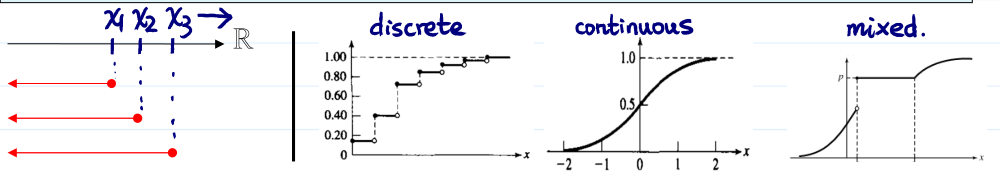
\includegraphics[width=0.8\textwidth]{image/cdf.png}
\end{figure}

\begin{definition}[概率质量函数]
    当且仅当函数$p(x)$满足下述条件时, 被称为\textbf{概率质量函数}(probability mass function, p.m.f.):
    \begin{itemize}
        \item $p(x)\ge 0$
        \item $\sum_{x \in \X}p(x)=1$
    \end{itemize}
\end{definition}

当$X$是离散型随机变量, 设$\mathscr{F}_{\mathcal{X}}$由$\mathcal{X}$的所有子集组成, 此时$X$的分布由
\[ p_{X}(x) = \P\{X=x\} = \P(\{\omega\in\Omega:X(\omega)=x\}), \quad x\in\mathcal{X} \]
唯一刻画. 其与分布函数间的关系为:
\begin{itemize}
    \item $F(x) = \sum_{t\le x}P(X=t)=\sum_{t\le x}p(t)$
    \item $p(x)=P(X=x)=F(x)-F(x-)$
\end{itemize}

\begin{definition}[概率密度函数]
    当且仅当函数$f(x)$满足下述条件时, 被称为\textbf{概率密度函数}(probability density function, p.d.f.):
    \begin{itemize}
        \item $f(x)\ge 0$
        \item $\int_{-\infty}^{\infty}f(x)=1$
    \end{itemize}
\end{definition}

当$X$是连续型随机变量, 且$F_{X} : \R^{n} \to [0,1]$可微(或者更一般地, \underline{绝对连续}), 此时$X$的分布由
\[ f_{X} := \frac{\partial^{n} F_{X}}{\partial x_{1} \cdots \partial x_{n}} \]
唯一刻画. 其与分布函数间的关系为:
\begin{itemize}
    \item $F(x) = \int_{-\infty}^x f(t)dt$
    \item $f(x)=\frac{d}{dx}F(x)$
\end{itemize}

\begin{remark}
    即使对于$f(x)>0$的$x$, $P(X=x)=x\int_{x}^x f(t)dt=0$, 即连续型随机变量在实轴上任意一点的概率测度为零. 概率密度函数$f(x)$代表的是在此位置上单位长度的概率, 可能是一个很大的值.
\end{remark}

\section{多元随机变量}

\begin{definition}[随机向量]
    若随机变量$X_1(\omega), X_2(\omega),\cdots , X_n(\omega)$定义在\underline{同一概率空间}$(\Omega,\mathscr{F},\P)$上, 则称
    \[ X(\omega) = (X_1(\omega), X_2(\omega),\cdots , X_n(\omega)) \]
    构成一个n维\textbf{随机向量},亦称n维随机变量.
\end{definition}

\begin{proposition}
    若$B_n$为$\R^n$上任一博雷尔点集,有
    \[ \{ X(\omega) \in B_n \} \in \mathscr{F} \]
\end{proposition}

\begin{definition}
    称n元函数
    \[ F(x_1,x_2, \cdots , X_n)=\P \{ X_1(\omega)<x_1, X_2(\omega)<x_2,\cdots , X_n(\omega)<x_n \} \]
    为随机向量$X(\omega)$的\textbf{联合分布函数}(joint cdf).
\end{definition}

当$n=2$时,有
\begin{equation}\label{equ:2dim_Prob}
    \P((a_1,b_1)\le X < (a_2,b_2))=F(b_1,b_2)-F(a_1,b_2)-F(b_1,a_2)+F(a_1,a_2)
\end{equation}

\begin{property}
    多元分布函数的一些性质:
    \begin{enumerate}
        \item 单调性:关千每个变元是单调不减函数;
        \item \begin{align*}
                  F(x_1,x_2, \cdots, -\infty, \cdots, X_n)=0 \\
                  F(+\infty,+\infty, \cdots, , +\infty)=1
              \end{align*}
        \item 关于每个变元右连续.
        \item 在二元场合,还应该有:对任意$ a_1 <b,,a_2<b_2$ ,都有
              \[ F(b_1,b_2)-F(a_1,b_2)-F(b_1,a_2)+F(a_1,a_2)\ge 0   \]
    \end{enumerate}
\end{property}

为保证\ref{equ:2dim_Prob}式中的概率的非负性,性质4是必须的,而且由性质4可以推出单调性,但存在着反例说明,由单调性并不能保证性质4的成立(见习题 12) .这是多元场合与一元场合的不同之处.

\subsection{边际分布}

\begin{definition}
    对于多维随机变量$X$, 只考虑其中一个分量的分布时, 称其为$X$的\textbf{边际分布或边缘分布}. 对于分量$X_i$, 其\textbf{边缘分布函数}(marginal cdf)为:
    \[ F_{X_i}(x_i) = \P\{ X_i \le x_i \} = F(\infty,\cdots , x_i ,\cdots ,\infty)\]
\end{definition}



\subsection{独立}

\begin{definition}[独立随机变量]
    若随机变量$X(\omega) = (X_1(\omega), X_2(\omega),\cdots , X_n(\omega))$联合分布函数可分解成各分量边缘分布函数的乘积, 即:
    \[ F(x_1,x_2,\cdots ,x_n) = F_{X_1}(x_1)F_{X_2}(x_2)\cdots F_{X_n}(x_n) , \quad \forall x_1,x_2,\cdots ,x_n \in \R \]
    则称随机变量$X$各分量相互\textbf{独立}
\end{definition}

\begin{remark}
    对于一般的多元随机变量, 其各分量边缘分布不足以描述联合分布的情况. 但若其各分量独立则可以.
\end{remark}

\begin{theorem}
    对于连续情况:
    \begin{align*}
                        & F(x_1,x_2,\cdots ,x_n) = F_{X_1}(x_1)F_{X_2}(x_2)\cdots F_{X_n}(x_n) \\
        \Leftrightarrow & f(x_1,x_2,\cdots ,x_n) = f_{X_1}(x_1)f_{X_2}(x_2)\cdots f_{X_n}(x_n)
    \end{align*}
    对于离散情况:
    \begin{align*}
                        & F(x_1,x_2,\cdots ,x_n) = F_{X_1}(x_1)F_{X_2}(x_2)\cdots F_{X_n}(x_n) \\
        \Leftrightarrow & p(x_1,x_2,\cdots ,x_n) = p_{X_1}(x_1)p_{X_2}(x_2)\cdots p_{X_n}(x_n)
    \end{align*}
\end{theorem}

\begin{theorem}
    若随机变量$X,Y$独立, 则其变换$Z=g(X), W=h(Y)$也独立.

    泛化情况:若随机向量$\{X\}_n$各分类独立, 则其变换$\{Y\}_n=g(\{X\}_n)$各分类也独立.
\end{theorem}

\subsection{条件分布}

\begin{definition}
    对一切使 $P\left(Y=y_{j}\right)=p_{ \cdot j}=\sum_{i=1}^{+\infty} p_{i j}>0$ 的 $y_j$, 称
    \begin{equation}\label{eq:3.5.1}
        p_{i | j}=P\left(X=x_{i} | Y=y_{j}\right)=\frac{P\left(X=x_{i}, Y=y_{j}\right)}{P\left(Y=y_{j}\right)}
        =\frac{p_{i j}}{p_{\cdot j}}, \quad i=1,2, \ldots
    \end{equation}
    为给定 $Y=y_j$ 条件下 $X$ 的条件分布列. 若$p_X(x)=0$, 则定义其为0.
\end{definition}

设二维连续随机变量 $(X,Y)$ 的联合密度函数为 $p(x,y)$, 边际密度函数为 $p_X(x),p_Y(y)$.

在离散随机变量场合, 其条件分布函数为 $P(X\leq x|Y=y)$. 但是, 因为连续随机变量取某个值的概率为零, 即 $P(Y=y)=0$, 所以无法用条件概率直接计算 $P(X\leq x|Y=y)$, 一个很自然的想法是: 将 $P(X\leq x|Y=y)$ 看成是 $h\to 0$ 时 $P(X\leq x|y\leq Y\leq y+h)$ 的极限, 即
\begin{align*}
    P(X \leq  x | Y=y) & =\lim _{h \to 0} P(X \leq  x | y \leq  Y \leq  y+h)                                                  \\
                       & =\lim _{h \to 0} \frac{P(X \leq  x, y \leq  Y \leq  y+h)}{P(y \leq  Y \leq  y+h)}                    \\
                       & =\lim _{h \to 0} \frac{\int_{-\infty}^{x} \int_{y}^{y+h} p(u, v) dv du}{\int_{y}^{y+h} p_{Y}(v) dv}  \\
                       & =\lim _{h \to 0} \frac{\int_{-\infty}^{x} \left\{ \frac{1}{h} \int_{y}^{y+h} p(u, v) dv \right\} du}
    {\frac{1}{h} \int_{y}^{y+h} p_{Y}(v) dv}.
\end{align*}
当 $p_Y(y),p(x,y)$ 在 $y$ 处连续时, 由积分中值定理可得
\begin{align*}
     & \lim _{h \to 0} \frac{1}{h} \int_{y}^{y+h} p_{Y}(v) dv=p_{Y}(y), \\
     & \lim _{h \to 0} \frac{1}{h} \int_{y}^{y+h} p(u, v) dv=p(u, y).
\end{align*}
所以
\[
    P(X \leq x | Y=y)=\int_{-\infty}^{x} \frac{p(u, y)}{p_{Y}(y)} du.
\]
至此, 我们可以定义连续随机变量的条件分布如下.

\begin{definition}
    对一切使 $p_Y(y)>0$ 的 $y$, 给定 $Y=y$ 条件下 $X$ 的\textbf{条件分布函数}\index{T!条件分布函数}和
    \textbf{条件密度函数}\index{T!条件密度函数}分别为
    \begin{align}
         & F(x | y)=\int_{-\infty}^{x} \frac{p(u, y)}{p_{Y}(y)} du, \\
         & p(x | y)=\frac{p(x, y)}{p_{Y}(y)}.
    \end{align}
    同理对一切使 $p_Y(y)>0$ 的 $x$, 给定 $X=x$ 条件下 $Y$ 的条件分布函数和条件密度函数分别为
    \begin{align}
         & F(y | x)=\int_{-\infty}^{y} \frac{p(x, v)}{p_{X}(x)} dv \\
         & p(y | x)=\frac{p(x, y)}{p_{X}(x)}.
    \end{align}
\end{definition}

\begin{remark}
    对于每一个\underline{固定的$x$}, $p_{Y|X}(y|x)$是一个关于$y$的概率质量函数; $f_{Y|X}(y|x)$是一个关于$y$的概率密度函数
\end{remark}

与概率三定理的对应:
\begin{description}
    \item[乘法法则] $p_{XY}(x,y)=p_{Y|X}(y|x)p_{X}(x), \quad f_{XY}(x,y)=f_{Y|X}(y|x)f_{X}(x)$
    \item[全概率公式] $p_{Y}(y)=\sum_{x}p_{Y|X}(y|x)p_{X}(x), \quad f_{Y}(y)=\int^{+\infty}_{-\infty}f_{Y|X}(y|x)f_{X}(x)dx$
    \item[Bayes原理]  $p_{X|Y}(x|y)=\frac{p_{Y|X}(y|x)p_{X}(x)}{\sum_{x}p_{Y|X}(y|x)p_{X}(x)}, \quad f_{X|Y}(x|y)=\frac{f_{Y|X}(y|x)f_{X}(x)}{\int^{+\infty}_{-\infty}f_{Y|X}(y|x)f_{X}(x)dx}$
\end{description}

\section{随机变量的函数}

在统计学中,常需要转化原始数据以获取其中信息, 由此引出了研究随机变量的函数的需要.

\begin{theorem}[事件法]
    设$Y=g(X)$是随机向量$X=(X_1,X_2,\cdots ,X_n)$的函数, 则$Y$的分布由$X$的分布通过下式决定:
    \[ \P\{Y \in B\} = \P\{X \in A\}, \quad A=\{ \omega |g(\omega)\in B\} \]
\end{theorem}

此法是其他方法的基础, 但使用不便, 常用于离散随机变量.

\begin{example}\label{exp:sum_of_pmf}
    已知随机变量$X,Y$的联合概率质量函数为$p(x,y)$, 求$Z=X+Y$的分布
    \[ p_Z=P(Z=z)=P(X+Y=z)=\sum_{x=-\infty}^{\infty}p(x, z-x) \]

    若$X,Y$独立,则$p_Z(z)=\sum_{-\infty}^{\infty}p_X(x)p_Y(z-x)dx$, 为$p_X$与$p_Y$的卷积
\end{example}

\subsection{分布函数法}

通过下式获取随机变量的函数的分布:
\[ F_Y(y)=\begin{cases}
        \int_{A_y}f_X(x)dx \\
        \sum_{x \in A_y}p_X(x)
    \end{cases} , \quad A_y=\{ x|g(x)\le y \}
\]

对每一个变换分别运用上式则可得到向量函数的分布.

\begin{example}
    已知随机变量$X$的概率密度函数$f_X(x)$与分布函数$F_X(x)$, 求$Y=X^2$的分布
    \[ F_Y(y)=P(Y\le y)=P(-\sqrt{y}<X\le \sqrt{y})+P(X=\sqrt{y}=F_X(\sqrt{y})-F_X(-\sqrt{y}))+0 \quad y\ge 0\]

    \begin{align*}
        f_Y(y) =\frac{d}{dy}F_Y(y) & =\frac{d}{dy}F_X(\sqrt{y}) -\frac{d}{dy}F_X(\sqrt{y})                 \\
                                   & =f_X(\sqrt{y})\frac{1}{2\sqrt{y}} -f_X(-\sqrt{y})\frac{-1}{2\sqrt{y}} \\
                                   & =\frac{1}{2\sqrt{y}}(f_X(\sqrt{y})+f_X(-\sqrt{y}))
    \end{align*}

\end{example}

\begin{example}\label{exp:sum_of_pdf}
    已知随机变量$X,Y$的联合概率密度函数$f(x,y)$, 求$Z=X+Y$的分布
    \[ F_Y(y)=P(Y\le y)=P(-\sqrt{y}<X\le \sqrt{y})+P(X=\sqrt{y}=F_X(\sqrt{y})-F_X(-\sqrt{y}))+0 \quad y\ge 0\]

    \begin{align*}
        F_Z(z) & =P(Z\le z)=P(X+Y\le z)                                               \\
               & =\iint _{x+y\leqslant z}f(x,y)dxdy                                   \\
               & =\int_{-\infty}^{+\infty}\int_{-\infty}^{z-x}f(x,y)dxdy              \\
               & =\int_{-\infty}^{z}\int_{-\infty}^{\infty}f(x,v-x)dxdv, \quad y= v-x
    \end{align*}

    \[ f_Z(z)=\frac{d}{dz}F_Z(z)=\int_{-\infty}^{\infty}f(x,z-x)dx \]

    若$X,Y$独立,则$f_Z(z)=\int_{-\infty}^{\infty}f_X(x)f_Y(z-x)dx$, 为$f_X$与$f_Y$的卷积, 与\ref{exp:sum_of_pmf}类似
\end{example}

\begin{example}
    已知随机变量$X,Y$的联合概率密度函数$f(x,y)$, 求$Z=\frac{Y}{X}$的分布
    \[ Q_{z}=\{(x, y): y / x \leq z\}=\{(x, y): x<0, y \geq z x\} \cup\{(x, y): x>0, y \leq z x\} \]
    \begin{align*}
        F_{Z}(z) & =\iint_{Q_{z}} f(x, y) d x d y=\int_{-\infty}^{0} \int_{x z}^{\infty}+\int_{0}^{\infty} \int_{-\infty}^{x z} f(x, y) d y d x \\
                 & =\int_{-\infty}^{0} \int_{z}^{-\infty}+\int_{0}^{\infty} \int_{-\infty}^{z} x f(x, x v) d v d x \quad(\text{set} y=x v)      \\
                 & =\int_{-\infty}^{0} \int_{-\infty}^{z}(-x) f(x, x v) d v d x+\int_{0}^{\infty} \int_{-\infty}^{z} x f(x, xv) dvdx            \\
                 & =\int_{-\infty}^{z} \int_{-\infty}^{\infty}|x| f(x, xv) dxdv
    \end{align*}

    \[ f_Z(z)=\frac{d}{dz}F_Z(z)=\int_{-\infty}^{\infty}|x|f(x,xz)dx \]
\end{example}

\subsection{Copula}\label{subsec:Copula}
\begin{definition}
    设\underline{连续型}实值随机变量$X$有分布函数$F$, 易见$F$在$\overline{\R}=[-\infty,+\infty]$上从$0$递增到$1$. 定义相应的\textbf{分位数函数}(quantile function)为
    \[ F^{-1}(p) := \inf\{x\in\R:F(x)\ge p\}, \quad p \in [0,1]. \]
\end{definition}
\begin{remark}
    当$F$严格递增时, 这与一般的反函数定义相同.
\end{remark}

\begin{theorem}
    设\underline{连续型}实值随机变量$X$有分布函数$F$, 则$F(X) \sim \mathrm{Uniform}([0,1])$
\end{theorem}

\begin{proof}
    \[ \P\{F(X)\le p\} = \P\{X\le F^{-1}(p)\} = F(F^{-1}(p)) =p, \quad \forall p \in [0,1]. \]
\end{proof}

\begin{theorem}
    设\underline{连续型}实值随机变量$X$有分布函数$F$, 且设$U\sim\mathrm{Uniform}([0,1]) $, 则$ F^{-1}(U) \overset{d}{=} X$, 其中$\overset{d}{=}$表示分布相同(equal in distribution).
\end{theorem}

\begin{theorem}[Sklar定理]
    考虑多个\underline{连续型}实值随机变量$X_{1},\dots,X_{k}$, 记$X_{i}$的分布函数为$F_{i}$. 我们称$(F_{1}(X_{1}),\dots,F_{k}(X_{k}))$的分布函数$C : [0,1]^{k} \to [0,1]$为相应的\textbf{Copula}, 适合
    \[ C(F_{1}(x_{1}),\dots,F_{k}(x_{k})) = \P\{X_{1}\le x_{1},\dots,X_{k}\le x_{k}\}, \quad \forall x_{1},\dots,x_{k} \]
    这个结果称为\textbf{Sklar定理}
\end{theorem}


这个结果, 在金融统计中有颇多应用. 稍作诠释的话, Copula提取了变量间的\emph{相关性}, 通过粘合\emph{边际}能够恰好地表示\emph{总体}.
人们可以构造各种各样的Copula, 对真实世界进行建模.

\subsection{概率密度函数法}

\begin{theorem}
    设连续随机变量$X$的概率密度函数为$f_X(x)$. 令$Y=g(X)$, 其中$g$为可微函数, 且严格单调, 则当$y=g(x)$有定义时:
    \[ f_Y(y)=f_X(g^{-1}(y))\left| \frac{dg^{-1}(y)}{dy} \right|  \]
    否则为$0$

    若$g$为分段单调函数, 则\underline{分段}计算上是结果, 再进行相加
\end{theorem}

\begin{theorem}
    设连续随机向量$\mathbf{X}$的概率密度函数为$f_\mathbf{X}(\mathbf{x})$. 令$\mathbf{Y}=\mathbf{g}(\mathbf{X})$, 其中$\mathbf{g}$为双射, 定义其逆函数为:
    \[ \mathbf{x}=\mathbf{g}^{-1}(\mathbf{y})=\mathbf{w}(\mathbf{y}) \]
    若$\mathbf{w}$存在连续偏导数, 则当$\mathbf{Y}=\mathbf{g}(\mathbf{X})$有定义时:
    \[ f_\mathbf{Y}(\mathbf{y})=f_\mathbf{X}(\mathbf{g}^{-1}(\mathbf{y}))\left| \frac{\partial \mathbf{w}}{\partial \mathbf{y}} \right|  \]
    否则为$0$
\end{theorem}

\begin{remark}
    若$\mathbf{Y}$的维数$k$小于$\mathbf{X}$的维数$n$, 可增补$n-k$维的函数$\mathbf{Z}=\mathbf{h}(\mathbf{X})$, 使得$(\mathbf{Y},\mathbf{Z})$满足条件, 再通过积分获取$\mathbf{Y}$的概率密度函数.
\end{remark}

\begin{example}
    已知随机变量$X_1,X_2$的联合概率密度函数$f(x_1,x_2)$, 求$Y_1=\frac{X_2}{X_1}$的分布

    令$Y_{2}=X_{1}$, 则:
    \begin{align*}
        x_{1} & =y_{2}\equiv w_{1}(y_{1}, y_{2})       \\
        x_{2} & =y_{1} y_{2}\equiv w_{2}(y_{1}, y_{2})
    \end{align*}
    \[ \frac{\partial w_{1}}{\partial y_{1}}=0, \frac{\partial w_{1}}{\partial y_{2}}=1, \frac{\partial w_{2}}{\partial y_{1}}=y_{2}, \frac{\partial w_{2}}{\partial y_{2}}=y_{1}\]
    \[ J=\left|\begin{array}{cc}0 & 1 \\ y_{2} & y_{1}\end{array}\right|=-y_{2}\]
    所以:
    \[ f_{Y_1 Y_2}(y_1, y_2)=f_{X_1 X_2}(y_{2}, y_{1} y_{2})\left|y_2\right| \]
    \[ f_{Y_1}(y_1)=\int_{-\infty}^{\infty} f_{Y_{1} Y_{2}}\left(y_{1}, y_{2}\right) d y_{2}=\int_{-\infty}^{\infty} f_{X_{1} X_{2}}\left(y_{2}, y_{1} y_{2}\right)\left|y_{2}\right| d y_{2} \]
\end{example}

\subsection{矩母函数法}

\subsection{次序统计量}

\begin{definition}
    设$X_1,X_2,\dotsc,X_n$为随机变量, 将其按大小排序后记为$X_{(1)}\le X_{(2)} \le  \cdots \le X_{(n)}$, 则将$x_{(i)}$称为该样本的第$i$个\textbf{次序统计量}. 其中
    \begin{itemize}
        \item \textbf{最小次序统计量}定义为:$X_{(1)}=\min\{x_1,\dotsc,x_n\}$
        \item \textbf{最大次序统计量}定义为:$X_{(n)}=\max\{x_1,\dotsc,x_n\}$
        \item \textbf{极差}定义为:$R=X_{(n)}-X_{(1)}$
        \item 第$i$个\textbf{间差}定义为:$S_i=X_{(i)}-X_{(i-1)}$
    \end{itemize}
\end{definition}

\begin{remark}
    虽然$X_1,X_2,\dotsc,X_n$独立, 但其次序统计量一般不独立
\end{remark}

\begin{example}
    若$X_1,X_2,\dotsc,X_n$独立同分布, 求$X_{(1)}$与$X_{(n)}$的分布

    \begin{align*}
        F_{X_{(n)}}(x) & =P(X_{(n)} \leq x)=P(X_{1} \leq x, \ldots, X_{n} \leq x) \\
                       & =P(X_{1} \leq x) \cdots P(X_{n} \leq x)                  \\
                       & =[F(x)]^{n}                                              \\
        f_{X_{(n)}}(x) & = \frac{d}{dx}F_{X_{(n)}}(x)                             \\
                       & =nf(x)[F(x)]^{n-1}
    \end{align*}

    \begin{align*}
        1-F_{X_{(1)}}(x) & =P(X_{(1)}>x)=P(X_{1}>x, \ldots, X_{n}>x) \\
                         & =P(X_{1}>x)\cdots P(X_{n}>x)              \\
                         & =[1-F(x)]^{n}                             \\
        f_{X_{(1)}}(x)   & = \frac{d}{dx}F_{X_{(1)}}(x)              \\
                         & =nf(x)[1-F(x)]^{n-1}
    \end{align*}
\end{example}

\begin{theorem}
    第$i$个\textbf{次序统计量}的概率密度函数为:
    \[ f_{X_{(k)}} = C(n;1,k-1,n-k)f(x)[F(x)]^{k-1}[1-F(x)]^{n-k}  \]
\end{theorem}

\begin{figure}[!ht]
    \centering
    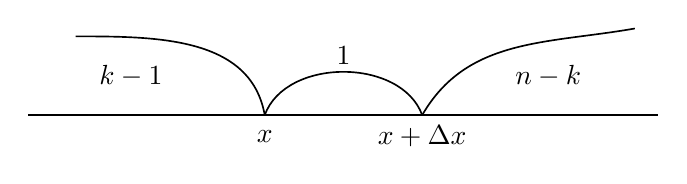
\begin{tikzpicture}[semithick]
        \draw(-4,0)--(4,0);\coordinate(a)at(-1,0);\node[below=2pt]at(a){$x$};
        \coordinate(b)at(1,0);\node[below]at(b){$x+\Delta x$};
        \draw[out=100,in=0](a)to(-3.4,1);
        \draw[out=70,in=110](a)to(b);
        \node at(0,0.75){$1$};\node at(-2.7,0.5){$k-1$};
        \draw[out=60,in=190](b)to(3.7,1.1);
        \node at(2.6,0.5){$n-k$};
    \end{tikzpicture}
    \caption{$X_{(k)}$取值的示意图}
\end{figure}

\begin{theorem}
    次序统计量$(x_{(i)},x_{(j)})(i<j)$的联合分布密度函数为
    \begin{align*}
        p_{ij}(y,z)=\frac{n!}{(i-1)!(j-i-1)!(n-j)!}[F(y)]^{i-1}[F(z)-F(y)]^{j-i-1} &   \\
        \cdot[1-F(z)]^{n-j}p(y)p(z),\quad y\leq z                                  & ,
    \end{align*}
\end{theorem}

\begin{proof}
对正$\Delta y,\Delta z$以及$y<z$,事件``$x_{(i)}\in(y,y+\Delta y],x_{(j)}\in(z,z+\Delta z]$''可以表示为``容量为$n$的样本$x_1,\dotsc,x_n$中有$i-1$个观测值小于等于$y$,一个落入区间$(y,y+\Delta y],j-i-1$个落入区间$(y+\Delta y,z]$,一个落入区间$(z,z+\Delta z]$,而余下$n-j$个大于$z+\Delta z$''(见图~\ref{fig:5.3.6} ).
\begin{figure}[!ht]
    \centering
    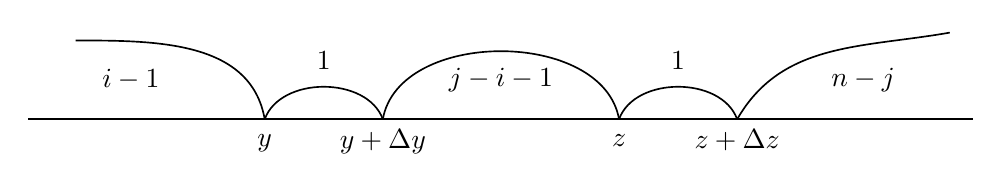
\begin{tikzpicture}[semithick]
        \draw(-6,0)--(6,0);
        \coordinate(a) at(-3,0);\coordinate(b)at(-1.5,0);
        \coordinate(c)at(1.5,0);\coordinate(d)at(3,0);
        \node[below=2pt]at(a){$y$};\node[below]at(b){$y+\Delta y$};
        \node[below=2pt]at(c){$z$};\node[below]at(d){$z+\Delta z$};
        \draw[out=100,in=0](a)to(-5.4,1);
        \draw[out=70,in=110](a)to(b);\draw[out=70,in=110](c)to(d);
        \node at(-2.25,0.75){$1$};\node at(-4.7,0.5){$i-1$};
        \draw[out=60,in=190](d)to(5.7,1.1);
        \node at(4.6,0.5){$n-j$};\node at(0,0.5){$j-i-1$};
        \draw[out=80,in=100](b)to(c);
        \node at(2.25,0.75){$1$};
    \end{tikzpicture}
    \caption{$x_{(i)}$与$x_{(j)}$取值的示意图}\label{fig:5.3.6}
\end{figure}
\end{proof}
\begin{example}
    若$X_1,X_2,\dotsc,X_n$独立同分布, 求$R=X_{(n)}-X_{(1)}$的分布

    \[ f_{X_{(1)}X_{(n)}}(s,t)=n(n-1)f(s)f(t)[F(t)-F(s)]^{n-2}\mathbb{I}(s\le t) \]

    \[ f_R(r)=\mathbb{I}(r>0)\int_{-\infty}^{\infty}f_{X_{(1)}X_{(n)}}(s,s+r)ds \]

\end{example}
\chapter{随机变量的数值特征}

\section{期望}

\begin{definition}
    对于实值随机向量$X : (\Omega,\mathscr{F},\P) \to (\R,\mathscr{B}_{\R})$和(可测)函数$g : \Rn \to \R$, 称
    \[ \E[g(X)] = \int_{\Omega} g(X(\omega))\,\d\P(\omega) = \int_{\R} g(x) \,\d F_{X}(x) \]
    为$g(X)$的\textbf{期望}(expectation).
\end{definition}

\begin{remark}
    当$F_{X}(x)$在$x_0$出连续可导时, $\d F_{X}(x_0)=f_{X}(x_0)\d x$; 当$x_0$为其间断点时时, $\d F_{X}(x_0)=p_{X}(x_0)\delta(x_0)\d x$
\end{remark}

期望算子$\E$是一个线性泛函, 仅适用于\underline{可积}的随机变量.

\begin{definition}
    \begin{enumerate}
        \item 当$g(x)=x$时, $\E[g(x)]=\E[X]$称作$X$的\textbf{均值}(mean), 记为$\mu_{X}$
        \item 当$g(x)=(x-\mu_{X})^{2}$时, $\E[g(x)]=\E[(X-\E[X])^{2}]$称作$X$的\textbf{方差}(variance), 记为$\sigma^2_{X}$. 其平方根称作$X$的\textbf{标准差}(standard deviation), 记为$\sigma_{X}$
        \item 当$g(x,y)=(x-\mu_{X})(y-\mu_{Y})$时, $\E[g(X,Y)]=\E[(X-\E[X])(Y-\E[Y])]$称作$X$与$Y$的\textbf{协方差}(covariance), 记为$\Cov(X,Y)$或$\sigma_{XY}$.
        \item 定义$X$与$Y$的\textbf{相关系数}(correlation coefficient)为:$\sigma_{XY}/(\sigma_{X}\sigma_{Y})$, 记为$\Cor(X,Y)$或$\rho_{XY}$. 若$\rho_{XY}=0$, 则称$X$与$Y$不相关
    \end{enumerate}
\end{definition}

\subsection{均值}

\begin{remark}
    \begin{itemize}
        \item 随机变量的均值可看作其加权平均, 权重为其pdf或pmf, 也即其质心. 从大数定律(\ref{chap:limitation})的角度看, 也可解释为其长期均值.
        \item 方差为随机变量距其均值的均方偏差, 刻画了$X$的变动程度
        \item 随机变量的均值与标准差的单位和其本身的相同, 方差的为其平方
    \end{itemize}
\end{remark}

\begin{theorem}
    均值为随机变量的线性映射, 即:
    \[ \E(a+\sum_{i=1}^n b_i X_i)=a+\sum_{i=1}^n b_i\E( X_i) \]
\end{theorem}

\begin{theorem}[]
    若$X,Y$独立,则
    \begin{gather*}
        \E(XY)=\E(X)\E(Y)
        \E(g(X)h(Y))=\E(g(X))\E(h(Y))
    \end{gather*}
\end{theorem}

\begin{remark}
    由于$\E(X/Y)= \E(X)\E(\frac{1}{Y})$, 而$\E(\frac{1}{Y}) \neq \frac{1}{\E(Y)}$, 所以$\E(X/Y)\neq \E(X)/\E(Y)$
\end{remark}

\begin{theorem}
    若$g$为\underline{下凸(convex)函数}, 则$\E[g(X)] \ge g[\E(X)]$; 若$g$为\underline{上凸(concave)函数}, 则$\E[g(X)] \le  g[\E(X)]$;
\end{theorem}

\begin{figure}
    \centering
    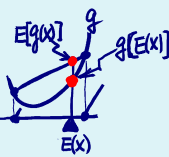
\includegraphics{image/trans_mean.png}
\end{figure}

一个重要结果是, 若$g(X) \ge 0$, 则$\E[g(X)] = 0 \implies g(X) \overset{\as}{=} 0$, 即$\P\{g(X)=0\} = 1$. 其证明可通过\textbf{Markov不等式}
\[ \P\{g(X)\ge\e\} \le \E[g(X)]/\e, \quad \forall \e > 0 \]
完成, 其中需要用到概率的\emph{连续性}, 即$\lim\limits_{n\to\infty}A_{n} = A \implies \lim\limits_{n\to\infty}\P(A_{n}) = \P(A)$.

预处理随机变量有两个常用变换:
\begin{itemize}
    \item \textbf{中心化}(centralization) $X \mapsto X-\E{X}$;
    \item \textbf{标准化}(standardization) $X \mapsto \dfrac{X-\E{X}}{\sqrt{\Var(X)}}$.
\end{itemize}

\subsection{方差}

\begin{theorem}
    $\sigma^2_X=\operatorname{Var}(X)=\E[(X-\mu_X)^2]=E(X^2)-\mu_X$
\end{theorem}

\begin{theorem}
    \[ \operatorname{Var}(a+bX)=b^2\operatorname{Var}(X) \]
\end{theorem}

\begin{theorem}
    \[ \operatorname{Var}(a+\sum_{i=1}^n b_i X_i)=\sum_{i=1}^n b_i^2 \operatorname{Var}(X_i)+\mathbf{b}^{\mathrm{T}} \Sigma \mathbf{b}\]
    其中$\Sigma$为协方差矩阵, $\Sigma_{i,j}=\operatorname{Cov}(X_i,X_j)$
\end{theorem}

\begin{theorem}
    若$X_1,\cdots ,X_n$相互独立, 则:
    \[ \operatorname{Var}(\sum_{i=1}^n X_i)=\sum_{i=1}^n\operatorname{Var}( X_i) \]
\end{theorem}

考虑\textbf{均方误差}(mean squared error)
\[ \MSE(X;\theta) = \E[|X-\theta|^{2}], \quad \theta\in\R, \]
通过\textbf{方差偏差分解}(variance-bias decomposition)
\[ \MSE(X;\theta) = \Var(X) + |\E{X}-\theta|^{2} \]
可以说明$\theta\mapsto\MSE(X;\theta)$在$\E{X}$处取到最小值$\Var(X)$.

\emph{投影}(projection)和\emph{正交分解}的思想在各种内积空间中应用广泛, 这里是$\E = \proj{}{\R}$, 概率论中关于子事件域$\mathscr{G}$ (随机元$X$, resp.)的\emph{条件期望}几何直观是$\proj{}{\mathscr{G}}$ ($\proj{}{\sigma(X)}$, resp.), 线性模型$\mathbf{y} = \mathbf{X}\bm{\beta} + \bm{\e}$中\emph{拟合值}为$\hat{\mathbf{y}} = \proj{\mathbf{y}}{\operatorname{Col}(\mathbf{X})}$.

\begin{theorem}[Chebyshev不等式]
    设随机变量$X$的均值与方差分别为:$\mu, \sigma^2$, 则:
    \[ \P(\left| X-\mu \right| >t)\le \frac{\sigma^{2}}{t^{2}} \]
\end{theorem}

\begin{proof}
    设$f(x)$为$X$的概率密度函数, 令$R=\left\{ x:|x-\mu|>t \right\} $
    \begin{align*}
        \P(|x-\mu|>t) & = \int_R 1 \cdot  f(x)\d x \le \int_R \frac{(x-\mu)^2}{t^{2}}f(x) \d x \\
                      & \le \int_{-\infty}^{\infty}\frac{(x-\mu)^2}{t^{2}}f(x) \d x            \\
                      & = \frac{\sigma^{2}}{t^{2}}
    \end{align*}
\end{proof}

\begin{remark}
    若令$t=k\sigma$, 则$\P(\left| X-\mu \right| >k\sigma)\le \frac{1}{k^{2}}$, 即标准差可代表随机变量偏离均值的概率单位距离.
\end{remark}

\begin{corollary}
    \[ \operatorname{Var}(X)=0 \implies P(X=\mu)=1 \]
\end{corollary}

\subsection{协方差}

协方差代表了$X$与$Y$之间的联合变化倾向, 或者说他们间的相关程度, 但其间\underline{未必有}因果关系.

\begin{theorem}
    \[ \operatorname{Cov} (X,Y)=\E[(X-\mu_X)(Y-\mu_Y)]=\E(XY)-\mu_Y \mu_Y \]
\end{theorem}

\begin{theorem}
    \[ \operatorname{Cov}(a+\sum_{i=1}^n b_i X_i,c+\sum_{j=1}^m d_j Y_j) = \sum_{i=1}^n\sum_{j=1}^m b_i d_j \operatorname{Cov}(X_i,Y_i) = \mathbf{b}^{\mathrm{T}}\Sigma \mathbf{d}\]
\end{theorem}

\begin{theorem}
    独立是不相关的\textbf{充分条件}, 但不是必要条件
\end{theorem}

\begin{theorem}
    $-1\le \rho_{XY} \le 1$, 当且仅当$X$与$Y$间为线性关系时取等号
\end{theorem}

\begin{proof}
    %TODO
\end{proof}

\begin{theorem}
    平移与缩放随机变量都不影响其协方差, 即:
    \[ \left| \operatorname{Cov}(a+ b X,c +d Y) \right| = \left| Cor(X,Y) \right|  \]
\end{theorem}

\section{条件期望}

\begin{definition}
    若$h(Y)$在给定$X=x$下的条件分布(定义\ref{def:cond_dist})的数学期望存在,则定义其为\textbf{条件期望}如下:
    \[ E(h(Y)|X=x) =\begin{cases}
            \sum_{y} h(y) p_{Y|X}(y|x),                    & \text{离散情况} \\
            \int_{-\infty}^{+\infty} h(y) f_{Y|X}(y|x) d y & \text{连续情况}
        \end{cases}\]
\end{definition}

\begin{remark}
    条件期望$\E_{Y|X}(Y|x)$是关于给定变量$x$的函数,不随对应变量$Y$本身变动,但其单位与对应变量$Y$相同,可看作一条在$(X,Y)$平面的曲线。
\end{remark}

\begin{theorem}
    若随机变量$X,Y$独立,则:
    \[ \E_{Y|x}(Y|x)=\E_{Y}(Y) \]
\end{theorem}

\begin{proof}
    由\label{thm:indep_cmf}可知,若随机变量$X,Y$独立,则
    \begin{align*}
        p_{Y|X}(y|x)&=p_{Y}(y) \\
        f_{Y|X}(y|x)&=f_{Y}(y)
    \end{align*}
    所以$\E_{Y|x}(Y|x)=\E_{Y}(Y)$
\end{proof}

由直观感受亦可知:若$X,Y$独立,则$X$不通过任何与$Y$相关的信息,其条件期望亦当与原期望相同。

\begin{note}
    令$g(x)=\E(h(Y)|X=x)$,则$g(X)$是随机变量$X$的变换,也是随机变量,记为$\E(h(Y)|X)$
\end{note}

\begin{theorem}[重期望公式]
    \[ \E_X[\E_{Y|X}(h(Y)|X)] = \E_{Y}[h(Y)] \]
\end{theorem}

\begin{proof}
    %TODO
\end{proof}

\begin{theorem}
    联合期望公式:
    \[ E_{X,Y}=E_X E_{Y|X} = E_Y E_{X|Y} \]
    泛化情况:
    \[ E_{X,Y}[h(X,Y)]=E_X E_{Y|X}[h(X,Y)|X] = E_Y E_{X|Y}[h(X,Y)|Y] \]
\end{theorem}

\begin{theorem}[重方差公式]\label{thm:var_dec}
    随机变量$Y$的方差可作如下分解:
    \[ \operatorname{Var}_Y(Y)=\operatorname{Var}_X[E_{Y|X}(Y|X)] + E_X[\operatorname{Var}_{Y|X}(Y|X)] \]
\end{theorem}

\begin{figure*}
    \centering
    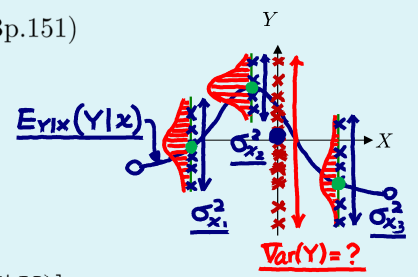
\includegraphics{image/var_dec.png}
\end{figure*}

\begin{corollary}
    \[ \operatorname{Var}_Y(Y) \ge E_X[\operatorname{Var}_{Y|X}(Y|X)] \]
    当且仅当$E_{Y|X}(Y|X)=E_Y(Y)$时取等号
\end{corollary}

\begin{figure*}
    \centering
    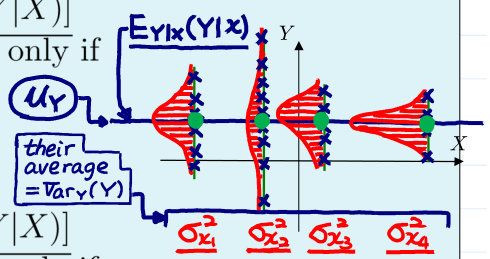
\includegraphics{image/var_dec2.png}
\end{figure*}

\begin{corollary}
    \[ \operatorname{Var}_Y(Y) \ge \operatorname{Var}_X[E_{Y|X}(Y|X)] \]
    当且仅当$\operatorname{Var}_{Y|X}(Y|X)=0$,即$\E_{Y|X}(Y|X)=Y$时取等号
\end{corollary}

\begin{figure*}
    \centering
    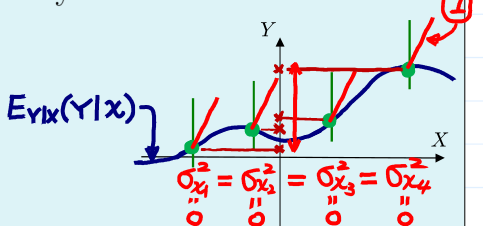
\includegraphics{image/var_dec3.png}
\end{figure*}

\section{矩母函数与特征函数}

\subsection{矩}

\begin{definition}
    对于随机变量$X$, 定义其$k$阶\textbf{矩}(moment)为$E(X^k)$, 记为$\mu_k$; 定义其$k$阶\textbf{中心矩}(central moment)为$E((X-\mu_X)^k)$, 记为$\upsilon_k$;
\end{definition}

易知矩与中心矩间存在以下关系:
\begin{align*}
    \upsilon_k & =\sum_{i=0}^k \binom{k}{i} \mu_i (-\mu_X)^{n-i}     \\
    \mu_k      & =\sum_{i=0}^k \binom{k}{i} \upsilon_i (\mu_X)^{n-i}
\end{align*}

特别的有:
\begin{align*}
    E(X)                  & =\mu_1                                                         \\
    \operatorname{Var}(X) & =\upsilon_2=\mu_1^2-2\mu_1 \cdot \mu_1 + \mu_2 = \mu_2-\mu_1^2
\end{align*}

\subsection{矩母函数}

\begin{definition}
    对于随机变量$X$, 若下式期望存在:
    \[ M_X(t) = \E(e^{tX}) \]
    则称其为\textbf{矩母函数}(moment generating function, mgf)。
\end{definition}

\begin{remark}
    此表达式等价于对概率质量函数或密度函数作Laplace变换, 当$t$取某些特定值时, 可能不存在. (若$t=0$则永远存在)
\end{remark}

\begin{theorem}
    若当$t$属于一个包含零点的开区间时, 矩母函数一直存在, 则其唯一对应一个概率分布.
\end{theorem}

\begin{theorem}
    若当$t$属于一个包含零点的开区间时, 矩母函数一直存在, 则:
    \[ M_X^{(k)}(0) = E(X^k) \]
\end{theorem}

\begin{remark}
    由此可方便地计算各阶矩, 故称其为矩母函数. 反过来, 若已知各阶矩, 通过Tayler展开式$M_X(t)=\sum_{k=0}^{\infty}\frac{M_X^{(k)}(0)}{k!}t^k$还原矩母函数, 进而得出概率分布.
\end{remark}

\begin{proposition}
    若$a,b$为常数, 则
    \[ M_{a+b X}(t) = e^{a t}M_X(b t) \]
\end{proposition}

\begin{theorem}
    若$X,Y$独立,则
    \[ M_{X+Y}(t) = M_X(t) M_Y(t) \]

    泛化情况: 若$X_1,\cdots, X_n$相互独立,则
    \[ M_{X_1+\cdots+ X_n} = \prod_{i=1}^n M_{X_i}(t)\]
\end{theorem}

\subsection{联合特征函数}

\begin{definition}
    对于随机变量$X_1,\cdots, X_n$, 若下式期望存在:
    \[ M_{X_1\cdots X_n}(t_1,\cdots ,t_n) = \E(e^{t_1 X_1+\cdots + t_n X_n}) \]
    则称其为\textbf{联合矩母函数}(joint moment generating function, joint mgf)。
\end{definition}

\begin{remark}
    此处为\underline{多元}函数
\end{remark}

\begin{proposition}
    \[ M_{X_i}(t_i) = M_{X_1\cdots X_n}(0,\cdots ,t_i,\cdots ,0) \]
\end{proposition}

\begin{theorem}
    当且仅当:
    \[ M_{X_1\cdots X_n}(t_1,\cdots ,t_n) = \prod_{i=1}^n M_{X_i}(t_i) \]
    时, $X_1,\cdots, X_n$相互独立
\end{theorem}

\begin{remark}
    与\underline{累计函数、密度函数、质量函数}的情况类似,变量相互独立等价于联合函数可拆分为边缘函数的乘积
\end{remark}

\begin{theorem}
    \[ \frac{\partial^{r_1+\cdots +r_n} }{\partial t_1^{r_1} \cdots  \partial t_n^{r_n}} M_{X_1\cdots X_n}(t_1,\cdots ,t_n) = E(X_1^{r_1} \cdots X_n^{r_n}) \]
\end{theorem}

\subsection{特征函数}

由于有时矩母函数可能不存在,为避免此缺陷,构造出与之特性类似的特征函数。

\begin{definition}
    对于随机变量$X$, 定义其\textbf{特征函数}(characat function, chf)为:
    \[ \phi_X(t) = \E(e^{itX}) = \E(\cos (tX)) + i\E(\sin (tX))\]

    对于随机变量$X_1,\cdots, X_n$, 定义其\textbf{联合特征函数}(joint characat function, joint chf)为:
    \[ \phi_{X_1\cdots X_n}(t_1,\cdots ,t_n) = \E(e^{i (t_1 X_1+\cdots + t_n X_n)}) \]
\end{definition}

\begin{remark}
    此表达式等价于对概率质量函数或密度函数作Fourier变换
\end{remark}

\begin{proposition}
    随机变量的特征函数总是存在
\end{proposition}

\begin{proposition}
    若矩母函数存在,则其与特征函数之间满足关系:
    \[ \phi_X(t) = M_X(it) \]
\end{proposition}

\begin{theorem}
    特征函数可通过以下逆变换得到分布:
    \begin{description}
        \item[离散] $p_{X}(x)=\lim _{T \rightarrow \infty} \int_{-T}^{T} e^{-i t x} \phi_{X}(t) d t$
        \item[连续] $f_{X}(x)=\frac{1}{2 \pi} \int_{-\infty}^{\infty} e^{-i t x} \phi_{X}(t) d t$
    \end{description}
\end{theorem}



\section{熵与信息}

\chapter{常见分布}

\section{离散分布}

\section{连续分布}

\section{正态分布及其导出分布}

\chapter{概率极限}\label{chap:limitation}
\begin{introduction}[考试重点]
    \item 收敛性
    \item Borel-Cantelli引理
    \item 各种概率不等式
    \item 特征函数在处理概率极限定理中的应用
    \item 各种大数定律及证明,如雷尔-康特立引理
    \item 中心极限定理
\end{introduction}
\section{收敛}

\begin{definition}
    若随机变量序列$\left\{ X_n: \Omega \to \mathbb{R} \right\}$与随机变量$X:\Omega \to \mathbb{R}$间存在以下关系:
    \[ \P\left\{ \omega \in \Omega: \lim_{n \to \infty}\abs{ X_n(\omega) - X(\omega)} < \epsilon \right\} =1, \forall \epsilon > 0\]
    则称$X_{n}$\textbf{几乎必然收敛}(converges almost surely)于$X$, 记为$X_{n} \xrightarrow{\as} X$。
\end{definition}

\begin{remark}
    类似于微积分中逐点收敛的条件。考察满足条件$\lim_{n \to \infty}\abs{ X_n(\omega) - X(\omega)} < \epsilon$的样本点,这些样本点组成事件的概率为1。
\end{remark}

% 若
%     \[ \P\{\lim\limits_{n\to\infty}X_{n} \neq X_{\infty}\} = 0
%         \iff \P\{\abs{X_{n}-X_{\infty}}>\e ~~\mathrm{i.o.}\} = 0, \ \forall \e>0 \]
%     \[ \hspace{2.33em} {\color{gray}(\text{利用概率$\P$的连续性})} ~\iff \lim_{N\to\infty}\P(\cup_{n=N}^{\infty}\{\abs{X_{n}-X_{\infty}}>\e\}) = 0, \ \forall \e>0 \]
% 注意$\{A_{n} ~~\mathrm{i.o.}\} = \{\sum_{n=1}^{\infty}\1_{A_{n}} = \infty\} = \bigcap_{N=1}^{\infty}\bigcup_{n=N}^{\infty} A_{n}$表示$A_{n}$发生\emph{无穷多次}(infinitely often). \vspace{0.2ex}


\begin{definition}
    若随机变量序列$\left\{ X_n: \Omega \to \mathbb{R} \right\}$与随机变量$X:\Omega \to \mathbb{R}$间存在以下关系:
    \[ \lim_{n\to\infty}\P\{\omega \in \Omega: \abs{X_n(\omega) - X(\omega)}<\e\} = 1, \ \forall \e>0. \]
    则称$X_{n}$\textbf{依概率收敛}(converges in probability)于$X$, 记为$X_{n} \xrightarrow{\P} X$。
\end{definition}

\begin{remark}
    即对于$Z_i$,事件$A_i=\{\omega \in \Omega: \abs{X_n(\omega) - X(\omega)}<\e\}$,$P(A_i)$将逐渐变为1。
\end{remark}

\begin{figure*}[h]
    \centering
    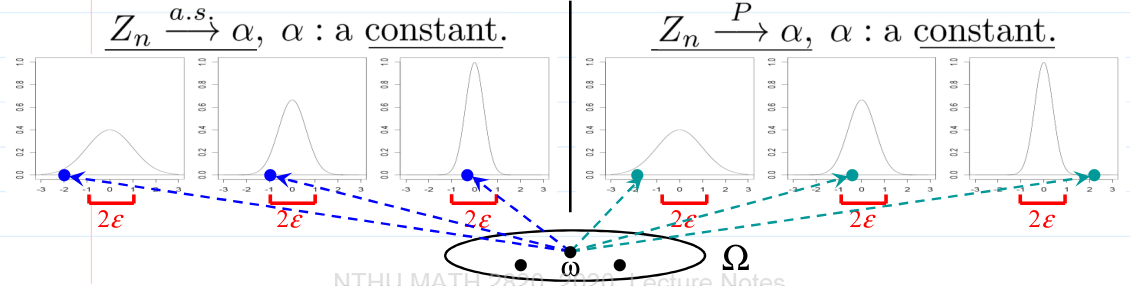
\includegraphics[width=0.9\textwidth]{image/converge1.png}
\end{figure*}

\begin{remark}
    对于几乎必然收敛的情况,每个样本点上的序列随机变量都在逐渐趋近收敛变量;而对于依概率收敛的情况,由于对某个样本点的概率为0(例如连续随机变量),可能某一次样本点的序列随机变量接近收敛变量,下一次又离开收敛变量,只有保证总体概率趋近1即可。
\end{remark}

易见$X_{n} \xrightarrow{\as} X_{\infty} \implies X_{n} \xrightarrow{\P} X_{\infty}$, 但是反之不成立, 例如概率空间$((0,1],\mathscr{B}_{(0,1]},\mathrm{Uniform}((0,1]))$上的\emph{打字机序列}
\[ \xi_{n} = \1_{(n/2^{k}-1,(n+1)/2^{k}-1]}, \quad 2^{k} \le n < 2^{k+1} \]
适合$\P\{\abs{\xi_{n}}>\e\} \le 1/2^{k} \to 0$, 而$\varlimsup \xi_{n} \equiv 1$且$\varliminf \xi_{n} \equiv 0$, 所以$\lim \xi_{n}(\omega)$对$\forall \omega \in (0,1]$都不存在.

\begin{proposition}
    依概率收敛是几乎必然收敛的\underline{必要条件},但\underline{不是充分条件}。
\end{proposition}

\begin{example}
    依概率收敛而不几乎必然收敛的实例:
    设样本空间为$\Omega = (0,1]$,概率均匀分布在样本空间上,即$P([a,b])=b-a,0<a<b<1$。接下来对于$k \in \mathbb{N}_+$,将区间$(0,1]$分为$2^{k}$个等长的子区间,并分别记为$I_{k,j}=(\frac{j-1}{2^k},\frac{j}{2^k}]$。

    按以下方式定义随机变量序列$\left\{ X_n: \Omega \to \mathbb{R} \right\}$:
    \[ X_n(\omega)=\begin{cases}
            1, \omega \in I_{k,j}    \\
            0, \omega \notin I_{k,j} \\
        \end{cases} ,\quad n = 2^k+j-2\]
    同时定义随机变量$X: \Omega \to \mathbb{R}$为$X(\omega)=0,\forall \omega \in \Omega$

    由于对任意$0<\epsilon<1$ 
    \[ \P\{\omega \in \Omega: \abs{X_n(\omega) - X(\omega)}<\e\}=1-\frac{1}{2^K} \to 1  \]
    所以$X_{n} \xrightarrow{\P} X$。
    然而对于任意$\omega \in \Omega$,无论k为何数,此次分割中,总有一个区间包含此样本点。即有无数个$X_i(\omega) = 1$。所以
    \[ \P\left\{ \omega \in \Omega: \lim_{n \to \infty}\abs{ X_n(\omega) - X(\omega)} < \epsilon \right\} =\P\{\emptyset \}=0 \]
    所以$X_{n}$不几乎必然收敛到$X$。
\end{example}

\begin{definition}
    设随机变量 $ X, X_1,  X_2, \dotsc $  的分布函数分别为 $ F (x), F_1 (x), F_2 (x), \dotsc $。若对 $ F (x) $ 的任一\underline{连续点} $x$, 都有
    \[ \lim_{n \to +\infty} F_n (x) = F (x) \]
    则称 $ \{ F_n (x) \} $ \textbf{弱收敛}于 $ F (x) $, 记作    $F_n (x) \xrightarrow{W}{\to} F (x)$;也称 $ \{ X_n \} $ 按\textbf{分布收敛}于$X$,记作$X_n \xrightarrow{d}{\to} X$
\end{definition}

\begin{proposition}
    依分布收敛是依概率收敛的\underline{必要条件},但\underline{不是充分条件}。但若依概率收敛到一个\underline{常数随机变量},则也可推出依分布收敛。
\end{proposition}

\begin{theorem}[连续映射定理]
    设$g: \mathbb{R}^k \mapsto \mathbb{R}$为\underline{连续}函数,则随机向量序列通过次映射后收敛情况与原先相同:
    \begin{align*}
        X_n^{(i)} \xrightarrow{\as} X^{(i)} &\Rightarrow g(X_n^{(1)},\cdots X_n^{(k)}) \xrightarrow{\as} g(X^{(1)},\cdots X^{(k)})\\
        X_n^{(i)} \xrightarrow{\P} X^{(i)} &\Rightarrow g(X_n^{(1)},\cdots X_n^{(k)}) \xrightarrow{\P} g(X^{(1)},\cdots X^{(k)})\\
        (X_n^{(i)}) \xrightarrow{d} (X^{(i)}) &\Rightarrow g(X_n^{(1)},\cdots X_n^{(k)}) \xrightarrow{d} g(X^{(1)},\cdots X^{(k)})\\
    \end{align*}
\end{theorem}
\begin{remark}
    随机向量依分布收敛是指\underline{联合}分布函数收敛。
\end{remark}

\begin{theorem}[Slutsky定理]\label{thm:Slutsky}
    若$X_n \xrightarrow{d} X, Y_n \xrightarrow{P} a$,其中$a$是常数,则:
    \begin{itemize}
        \item $Y_n X_n \xrightarrow{d} a X$
        \item $Y_n + X_n \xrightarrow{d} a + X$
        \item $\frac{X_n}{Y_n}  \xrightarrow{d} \frac{X}{a}$,若对所有的$n$都有$P(Y_n\neq 0)=1$,并且$a\neq 0$
    \end{itemize}
\end{theorem}

\begin{proof}
    由条件可知,$(X_n,Y_n) \xrightarrow{d} (X,a)$,且$g_1(X_n,Y_n)=X_n Y_n, g_2(X_n,Y_n)=X_n+Y_n, g_3(X_n,Y_n)=\frac{X_n}{Y_n}$都是连续函数($g_3$在定理中的限制下),所以仍然保持依分布收敛。
\end{proof}
\begin{remark}
    当$Y_n \xrightarrow{P} a$才能得出$(X_n,Y_n) \xrightarrow{d} (X,a)$;若$Y_n$依分布收敛到其他随机变量,则未必成立。
\end{remark}

\begin{theorem}[theta方法的极限定理]
    设
    \[ \frac{\sqrt{n}(X_n-\theta)}{\sigma} \xrightarrow{d} N(0,1) \]
    那么对于连续函数$g$,若$g'(\theta)\neq 0$存在,则
    \[ \frac{\sqrt{n}(g(X_n)-g(\theta))}{\sigma|g'(\theta)|} \xrightarrow{d} N(0,1) \]
\end{theorem}

\begin{proof}
    %TODO
\end{proof}

\begin{theorem}[连续性定理]\label{thm:continuity}
    设$F_n(x)$是一个累计函数序列,并且分别对应矩母函数$M_n(t)$;$F(x)$是一个累计函数,并且对应矩母函数$M(t)$。那么,
    \[ \forall t \in U(0,\delta) ,s.t. \lim_{n \to \infty}M_n(t) = M(t)\]
    是在$F(x)$的所有连续点上$F_n(x) \xrightarrow{M} F(x)$的充要条件。
\end{theorem}
\begin{remark}
    若矩母函数不存在,替换成特征函数,定理也成立。但是,不能替换成密度函数或质量函数
\end{remark}

\begin{example}
    离散情况:\\
    设均匀随机变量$X_n \sim U(-\frac{1}{2},\frac{1}{2})$,那么$X_n \xrightarrow{d} 0$。然而$P_n(x) \to 0, \forall x \in \mathbb{R}$(不满足质量函数定义),并且$\lim_{n \to \infty}F_n(0)=\frac{1}{2}$(不满足累积函数定义)

    连续情况:\\
    设累积函数为$F_n(x)=x-\frac{\sin (2n\pi x)}{2n\pi}, 0<x<1$,那么$F_n \xrightarrow{d} U(0,1)$。然而$f_n(x)$无极限
\end{example}

\begin{example}[泊松分布收敛于正态分布]
    令$X_n \sim P(\lambda_n)$,并且$\lim_{n \to \infty}\lambda_n =\infty$。将变量标准化:
    \[ Z_n=\frac{X_n-\lambda_n}{\sqrt{\lambda_n}} \]
    那么
    \[M_{Z_n}(t)=\ee^{-t\sqrt{\lambda_n}}M_{X_n}(t)(\frac{t}{\sqrt{\lambda_n}})=\exp (-t\sqrt{\lambda_n}+\lambda_n(e^{\frac{t}{\sqrt{\lambda_n}}-1}))\]
    由于
    \[ \lim_{n \to \infty}\ln (M_{Z_n}(t))=\lim_{\lambda_n \to \infty}-t\sqrt{\lambda_n}+\lambda_n(e^{\frac{t}{\sqrt{\lambda_n}}-1})=\frac{t^2}{2} \]
    所以$Z_n \xrightarrow{d} N(0,1)$,即若$\lambda$很大,可通过$N(\lambda,\lambda)$估计$P(\lambda)$
\end{example}

\section{大数定理}\label{sec:large_number}

\begin{theorem}[弱大数定理]
    设随机变量$X_1,\cdots ,X_n$相互独立,且$E(X_i)=\mu,\operatorname{Var}(X_i)=\sigma^2$,那么
    \[ \overline{X_n}=\frac{1}{n}\sum_{i=1}^n X_i \xrightarrow{\P} \mu \]
\end{theorem}

\begin{remark}
    柯西分布无均值、方差,不能使用此定理。
\end{remark}

\begin{proof}
    易知
    \[ E(\overline{X_n})=\mu,\operatorname{Var}(\overline{X_n})=\frac{\sigma^2}{n} \]
    再通过切比雪夫不等式有:
    \[ P(\left\vert \overline{X_n}-\mu \right\vert >\epsilon)<\frac{\operatorname{Var}(\overline{X_n})}{\epsilon^{2}}=\frac{\sigma^2}{n \epsilon^2} \to 0 \]
\end{proof}

\begin{theorem}[强大数定理]
    设随机变量$X_1,\cdots ,X_n$相互独立,且$E(X_i)=\mu,\operatorname{Var}(X_i)=\sigma^2$,那么
    \[ \overline{X_n}=\frac{1}{n}\sum_{i=1}^n X_i \xrightarrow{\as} \mu \]
\end{theorem}

\begin{example}[蒙特卡洛积分]
    为计算积分$I(f)=\int_0^1 f(x)\mathrm{d}x$,生成随机数$X_1,\cdots ,X_n \operatorname{i.i.d.} \sim U(0,1)$,并且计算$\hat{I}(f)=\overline{Y_n}, Y_i=f(X_n) $。由于$X_1,\cdots ,X_n \operatorname{i.i.d.}$,所以$Y_1,\cdots ,Y_n \operatorname{i.i.d.}$;并且$E(Y_i)=E(f(X_i))=\int_0^1 f(x)\cdot 1\mathrm{d}x=I(f)$,所以$\hat{I}(f)\xrightarrow{\P} E(Y_i)=I(f)$
\end{example}

\begin{example}[样本方差]\label{ex:sample_var}
    设随机变量$X_1,\cdots ,X_n \operatorname{i.i.d.}$,并且均值和方差分别为$\mu,\sigma$。令:
    \[ S_n^2=\frac{1}{n}\sum_{i=1}^n(X_i-\overline{X_n}) = (\frac{1}{n}\sum_{i=1}^nX_i^2)-\overline{X_n}^2 +\]
    由于$g(x)=x^2$是连续函数,所以$\overline{X_n}^2 \xrightarrow{\P} \mu^2$。由于$X_1^2,\cdots X_n^2 \operatorname{i.i.d.}$,且$E(X_i^2)=\sigma^2+\mu^2$,所以$\overline{X_n^2} \xrightarrow{\P} \mu^2+\sigma^2$。因此:
    \[ S_n^2 \xrightarrow{\P}\mu^2+\sigma^2-\mu^2= \sigma^2 \]
\end{example}

\begin{example}\label{ex:t_disc_to_normal}
    若$X_n \sim t_n$,则$X_n \xrightarrow{d} N(0,1)$。
    令$Z \sim N(0,1),U_1,\cdots ,U_n \sim \chi^2_1$相互独立,则$\frac{Z}{\sqrt{(U_1+\cdots+U_n)/n}} \sim t_n$。由于$E(U_i)=1$,所以$\overline{U_n} \xrightarrow{\P} 1$,所以$\sqrt{\overline{U_n}} \xrightarrow{\P} 1$,所以$t_n=\frac{Z}{\sqrt{\overline{U_n}}} \xrightarrow{d} N(0,1)$(定理\ref{thm:Slutsky})。
\end{example}

\begin{example}
    若$X_n \sim F_{m,n}$,则$mX_n \xrightarrow{d} \chi^2_m$。
    令$U \sim \chi^2_m,V_1,\cdots ,V_n \sim \chi^2_1$相互独立,则$\frac{U/m}{(V_1+\cdots+V_n)/n} \sim F_{m,n}$。由于$E(V_i)=1$,所以$\overline{V_n} \xrightarrow{\P} 1$,所以$mF_{m,n}=\frac{U}{\overline{V_n}} \xrightarrow{d} \chi^2_m$(定理\ref{thm:Slutsky})。
\end{example}

\section{中央极限定理}

\begin{theorem}[中央极限定理]\label{thm:central_limit}
    设随机变量$X_1,\cdots ,X_n,\operatorname{i.i.d.}$,且$E(X_i)=\mu,\operatorname{Var}(X_i)=\sigma^2$,令
    \[ \overline{X_n} = \frac{1}{n}\sum_{i=1}^n X_i, T_n=\sum_{i=1}^n X_i\]
    则:
    \[ \lim_{n \to \infty}P(\frac{T_n-n \mu}{\sigma\sqrt{n}}\le x)=\lim_{n \to \infty}P(\frac{\sqrt{n}(\overline{X_n}-\mu)}{\sigma}\le x) =\Phi(x)\]
    其中$\Phi(x)$是$N(0,1)$的累积函数,即:
    \[ \frac{T_n-n \mu}{\sigma\sqrt{n}}=\frac{\sqrt{n}(\overline{X_n}-\mu)}{\sigma} \xrightarrow{d} N(0,1)\]
\end{theorem}

\begin{proof}
    令$W_i=\frac{X_i-\mu}{\sigma}$,则$E(W_i)=0,\operatorname{Var}(W_i)=1$。再令$Z_n=\frac{T_n-n \mu}{\sigma\sqrt{n}}=\frac{1}{\sqrt{n}}\sum_{i=1}^n W_i$。则
    \begin{align*}
        M_{Z_n}(t) &= \left[ M_{W}(\frac{t}{\sqrt{n}}) \right]^n \\
        &= \left[ M_{W}(0)+M_{W}'(0)\frac{t}{\sqrt{n}}+\frac{M_{W}''(0)}{2}(\frac{t}{\sqrt{n}})^2 +o(\frac{1}{n}) \right]^n \\
        &= \left[ 1 + \frac{t^2}{2n}+ o(\frac{1}{n}) \right]^n\\
        & \to e^{\frac{t^2}{2}}
    \end{align*}
    根据定理\ref{thm:continuity},$Z_n \xrightarrow{d} N(0,1)$。
\end{proof}
\begin{remark}
    若矩母函数不存在,可替换为特征函数。
\end{remark}

\begin{example}[二项分布近似为正态分布]
    若随机变量$X_1,\cdots ,X_n \operatorname{i.i.d.} \sim B(1,p)$, 则$T_n \sim B(n,p)$. 其中$E(T_n)=nE_(X_i)=np, \operatorname{Var}(T_n)=n\operatorname{Var}(X_i)=np(1-p)$. 根据中央极限定理有:
    \[ \frac{T_n - np}{\sqrt{np(1-p)}} \xrightarrow{d} N(0,1) \]
    即当n很大时, $B(n,p)$可用$N(np,np(1-p))$近似.
\end{example}
\begin{remark}
    其他与二项分布一样, 可以通过独立同分布的随机变量相加得到的分布,也可在一定条件下近似为正态分布. 例如Gamma分布(可通过指数分布相加得到), 泊松分布(泊松分布相加), 负二项分布(几何分布相加), 参见图\ref{fig:relationship_among_univariate_distributions}
\end{remark}
\begin{remark}
    由定理\ref{thm:Poisson_theorem}可知, 当$B(n,p)$中$n$很大$p$很小时, 二项分布可近似为泊松分布; 而泊松分布$\lambda$很大时, 又可近似为正态分布.
\end{remark}

\begin{example}[测量误差估计]
    假设每次测量结果为独立同分布的随机变量$X_1,\cdots ,X_n$, 其均值与方差分别为$\mu,\sigma^2$. 由中央极限定理可知$\frac{\sqrt{n}(\overline{X_n}-\mu)}{\sigma} \xrightarrow{d} N(0,1)$. 由例\ref{ex:sample_var}可知$S_n^2 \xrightarrow{\P} \sigma^2$, 即$\frac{\sigma}{S_n} \xrightarrow{\P} 1$(定理\ref{thm:Slutsky}). 所以:
    \[ \frac{\sqrt{n}(\overline{X_n}-\mu)}{S_n}=\frac{\sqrt{n}(\overline{X_n}-\mu)}{\sigma}\frac{\sigma}{S_n} \xrightarrow{d} N(0,1)\cdot 1=N(0,1) \]
    即可以通过分布$N(0,\frac{S_n^2}{n})$估计测量误差$\overline{X_n}-\mu$
\end{example}
\begin{remark}
    由定理\ref{thm:normal_sample_mean_variance}可知$\frac{\sqrt{n}(\overline{X_n}-\mu)}{S_n} \sim t_{n-1}$. 但由例\ref{ex:t_disc_to_normal}可知, $n\to \infty$时, $t$分布收敛于正态分布, 所以不冲突.
\end{remark}


\appendix

\chapter{基本数学工具}

\section{排列与组合}

全部组合分析公式的推导基于下列两条原理:
\begin{description}
    \item[乘法原理] 若进行$A_1$过程有$n_l$种方法,进行$A_2$过程有 $n_2$种方法,则进行$A_1$过程后再接着进行$A_2$程共有$n_1 \cdot  n_2$种方法
    \item[加法原理] 若进行$A_1$过程有$n_l$种方法,进行$A_2$过程有 $n_2$种方法,假定$A_1$过程与$A_2$过程是并行的,则进行过程$A_1$或过程$A_2$的方法共有$n_1 +n_2$种
\end{description}

排列与组合的定义及其计算公式如下.
\begin{enumerate}
  \item 排列:
  从 $n$ 个不同元素中任取 $r (r \le n)$ 个元素排成一列 (考虑元素先后出现次序),
  称此为一个排列,
  此种排列的总数记为 $P_n^r$,
  按乘法原理,
  取出的第一个元素有 $n$ 种取法,
  取出的第二个元素有 $n - 1$ 种取法\dots
  取出的第 $r$ 个元素有 $n - r + 1$ 种取法,
  所以有
  \begin{equation}
    P_n^r = n \times (n - 1) \times \dotsb \times (n - r + 1) = \frac{n!}{(n - r!)}.\label{eq1.2.2}
  \end{equation}
  若 $r = n$,
  则称为全排列,
  记为 $_n$.
  显然,
  全排列 $P_n = n!$.

  \item 重复排列:
  从 $n$ 个不同元素中每次取出一个,
  放回后再取下一个,
  如此连续取 $r$ 次所得的排列称为重复排列,
  此种重复排列数共有 $n^r$ 个.
  注意这里的 $r$ 允许大于 $n$.

  \item 组合:
  从 $n$ 个不同元素中任取 $r (r \le n)$ 个元素并成一组 (不考虑元素间的先后次序),
  称此为一个组合,
  此种组合的总数记为 $\binom{n}{r}$ 或 $C_n^r$.
  按乘法原理此种组合的总数为
  \begin{equation}
    \binom{n}{r} = \frac{P_n^r}{r!} = \frac{n (n - 1) \dotsb (n - r + 1)}{r!} = \frac{n!}{r! (n - r)!}.\label{eq1.2.3}
  \end{equation}
  在此规定 $0! = 1$ 与 $\binom{n}{0} = 1$.

  \item 重复组合:
  从 $n$ 个不同元素中每次取出一个,
  放回后再取下一个,
  如此连续取 $r$ 次所得的组合称为重复组合,
  此种重复组合总数为 $\binom{n + r - 1}{r}$.
  注意这里的 $r$ 也允许大于 $n$.
\end{enumerate}

上述四种排列组合及其总数计算公式,
在确定概率的古典方法中经常使用,
但在使用中要注意识别有序与无序、重复与不重复。

\end{document}